\documentclass[12pt, a4paper, oneside]{article}
\usepackage[francais]{babel}
\usepackage[T1]{fontenc}
\usepackage[utf8]{inputenc}
\usepackage{graphicx}
\usepackage{xcolor}
\usepackage{hyperref} 
\usepackage{glossaries} 

\begin{document}

\begin{figure}
    
\includegraphics[width=4cm]{logolemansU.png}
    \hfill
    
\includegraphics[width=4cm]{logo_IC2.png}
\end{figure}


\title{\color{blue}\textbf{Le Mans Université} \\
        \color{black} Licence Informatique 2ème année \\
       Module 174UP02 Rapport de Projet \\
       \textbf{Othello}}
\author{Péan Alexandra, Nasreddine Biya, Aly Rida Mahjoub, \\ Chaosok Kong, Meriem Taieb Kherafa}
\date{\today}

\maketitle

\newpage
\tableofcontents

\newpage

\section{Introduction}
   
Ce document présente un projet de jeu Othello réalisé dans le cadre de la 
    formation de Licence 2 Informatique à l’Université du Mans, pendant la 
    période de janvier à avril 2025. Ce projet a été développé en langage C avec 
    la bibliothèque SDL. Othello est un jeu de société composé d’un plateau de 
    jeu (appelé \textit{othellier}) et de 128 pions blancs et noirs. Les joueurs 
    jouent à tour de rôle après avoir chacun choisi une couleur. À la fin de la 
    partie, le joueur ayant le plus de pions de sa couleur sur le plateau est 
    déclaré vainqueur.\\

    Ce projet a pour objectif de mettre en pratique les connaissances acquises 
    dans plusieurs domaines : la programmation en C, la gestion de projet, la 
    conception d’algorithmes, et le développement d’interfaces graphiques. À 
    travers ce jeu, nous avons pu explorer des aspects techniques variés tels que 
    la logique de jeu, l’intelligence artificielle, la gestion d’un mode réseau, 
    et l’intégration d’une interface graphique. \\

    Le rapport se structure comme suit : dans une première partie, nous 
    présenterons le jeu, les scénarios d’utilisation ainsi que les principales 
    fonctionnalités. Dans une deuxième partie, nous détaillerons l’organisation 
    du projet, en expliquant la répartition des tâches et les outils utilisés 
    pour faciliter le travail collaboratif. Dans la troisième partie, nous 
    traiterons des différentes étapes du développement : gestion des parties, 
    mode IA, interface graphique, et mode réseau. Enfin, nous présenterons les 
    résultats obtenus, suivis d’une conclusion qui mettra en lumière les points 
    forts, les limites de notre travail, les écarts entre la planification 
    initiale et le déroulement réel du projet, ainsi que les leçons tirées de 
    cette expérience. En annexe, nous fournirons un exemple de débogage et des 
    tests (jeux d’essai et cas de test) étant disponible dans le dépôt Git, dans 
    un répertoire dédié nommé \texttt{test}, ainsi que des captures d’écran 
    prises à différentes étapes du jeu.

\section{Conception}
    Dans cette première partie, nous allons présenter le but du jeu ainsi que les différentes fonctionnalités que nous avons 
    mises en place. 

    \subsection{Présentation du jeu}
    Othello est un jeu de stratégie à deux joueurs, qui se joue sur un plateau de 8 cases sur 8. Chaque joueur possède des pions de couleur noire ou blanche. Le but du jeu est de terminer la partie avec le plus grand nombre de pions de sa propre couleur. \\
    \textbf{Règles du jeu :}
    \begin{itemize}
        \item Le plateau commence avec 4 pions placés au centre : deux blancs et deux noirs, en croix.
        \begin{figure}[h]
            \begin{center}
            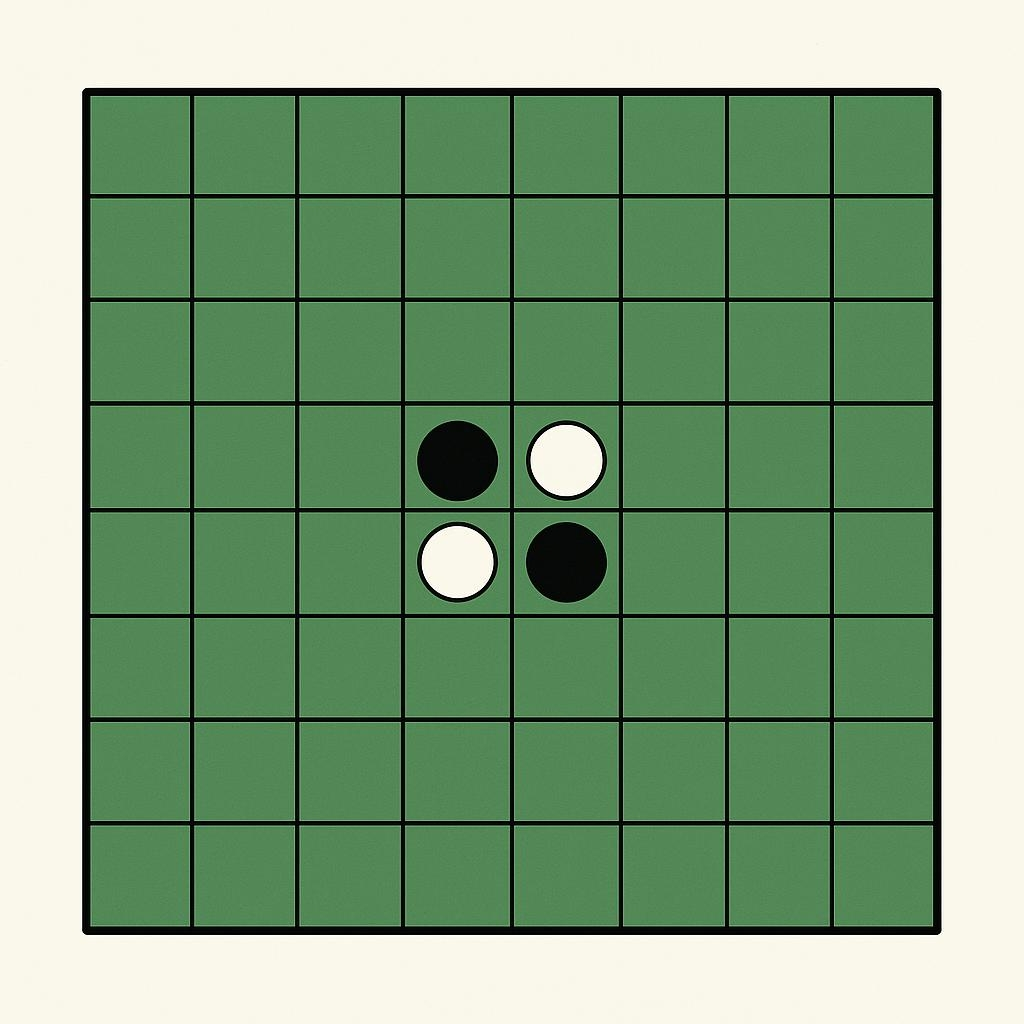
\includegraphics[height=5cm]{othello_depart_position.jpg}\\
            \caption{\textit{Position de départ}}
            \end{center}
            \end{figure}
        \item Les joueurs jouent à tour de rôle. Le joueur noir commence toujours.
        \item À chaque tour, un joueur place un pion de sa couleur sur une case vide de façon à encadrer un ou plusieurs pions adverses en ligne droite (horizontalement, verticalement ou en diagonale).
        \item Tous les pions adverses encadrés sont retournés et deviennent de la couleur du joueur.
        \item Si un joueur ne peut pas jouer, il passe son tour.
        \item La partie se termine quand le plateau est plein ou qu’aucun joueur ne peut jouer.
        \item Le joueur ayant le plus de pions de sa couleur sur le plateau à la fin gagne la partie.
    \end{itemize}    

    \subsection{Fonctionnalités}
        Lorsqu'on lance le jeu Othello, on arrive sur un menu principal proposant trois options. \\
        \begin{itemize}
        \item "Jouer" lance une nouvelle partie;
        \item "Partie sauvegardee" charge une partie existante depuis la liste des sauvegardes;
        \item "Quitter" ferme la fenêtre de jeu.
        \end{itemize}

Un bouton paramètres en haut à gauche du menu permet de personnaliser l'expérience. 
        Il est possible de modifier l'interface en choisissant entre un mode sombre et un 
        mode clair, ou d'ajuster le volume sonore. \\

Le bouton "jouer" ouvre sous menu demandant de choisir entre trois modes de jeu : \\
        \begin{itemize}
            \item "joueur vs joueur";
            \item "jouer en ligne";
            \item "joueur vs ordinateur".            
        \end{itemize}- 
        
        Si l'on choisit de jouer contre l'ordinateur, un second sous-menu apparaît pour sélectionner le niveau de difficulté, 
        suivi d'un autre choix permettant de déterminer la couleur des pions (blanc ou noir). Après avoir choisi ces options, 
        la partie commence. \\ \\

        Le plateau de jeu (othellier) est composé de 64 cases (8x8), sur lesquelles les joueurs placent leurs pions noirs ou blancs. 
        Pour faciliter la réflexion, les coups valides sont affichés automatiquement par un cercle non plein.\\
        
        Les pions posés sont des cercles pleins, noirs ou blancs. \\
        
        Les scores des joueurs sont affichés de chaque côté du plateau, indiquant le nombre de pions retournés. Un chronomètre 
        individuel est affiché de chaque côté du plateau. Il est activé uniquement pour les parties entre joueurs humains.
        Un indicateur de tour est affiché en haut du plateau. \\
        
        Un bouton "Sauvegarder" situé sous le plateau permet d'enregistrer la partie en cours. Une fois la sauvegarde effectuée, 
        le jeu redirige automatiquement vers le menu principal.\\

        Enfin, une musique à été ajouté dans le menu ainsi qu'un son de pion lorsqu'on joue une partie. 

\section{Organisation du projet}
    Cette partie présente la répartition des différentes tâches du projet dans le temps et parmi les membres du groupe, le déroulement
    classique de chaque séance de projet et les outils de gestion utilisés.
    
    \subsection{Répartition du travail}
    De manière synthétique, notre projet a été découpé en quatre tâches principales: \\
	\begin{itemize}
	    \item les fonctions de logique de jeu, c'est-à-dire celles qui assurent le déroulement d'une partie othello (poser un pion, changer de
    joueur, compter le score, etc.) y compris le système de sauvegarde;
	    \item l'interface graphique; 
	    \item l'algorithme intelligent pouvant affronter le joueur; 
            \item le mode multijoueur en ligne. 
	\end{itemize}
 
Dans un premier temps, la logique de jeu a été principalement conçue par Aly Rida, qui a codé la plupart des fonctions concernant la
pose des pions et la gestion du plateau. Meriem et Chaosok ont également contribué à cette première version du jeu, notamment en codant
une interface provisoire en terminal et un système de sauvegarde. \\

Nasreddine et Alexandra se sont formés à l'utilisation la bibliothèque SDL et, une fois la version console terminée, ont respectivement
créé le menu et l'interface graphique principale. Ce sont aussi eux qui ont adapté chaque nouvelle fonctionnalité à la version graphique
du projet au fur et à mesure de son développement. \\

L'étude des stratégies gagnantes en Othello et du modèle IA le plus adapté a été faite par Meriem, qui s'est ensuite chargée de coder
les fonctions liées à l'heuristique de l'IA ainsi que ses différents niveaux de difficulté. L'algorithme minmax a été implémenté par
Chaosok. Les différents niveaux de l'IA ont été testés de nombreuses fois par tous les membres du groupe afin d'évaluer la performance
de l'algorithme. \\

Ensuite, Aly Rida, Chaosok et Nasreddine ont travaillé sur la partie réseau: le mode multijoueur en local. Meriem et Alexandra ont
continué de corriger les bugs rencontrés dans la version offline du jeu et de rajouter les dernières modifications nécessaires.

        \begin{figure}[h]
            \begin{center}
            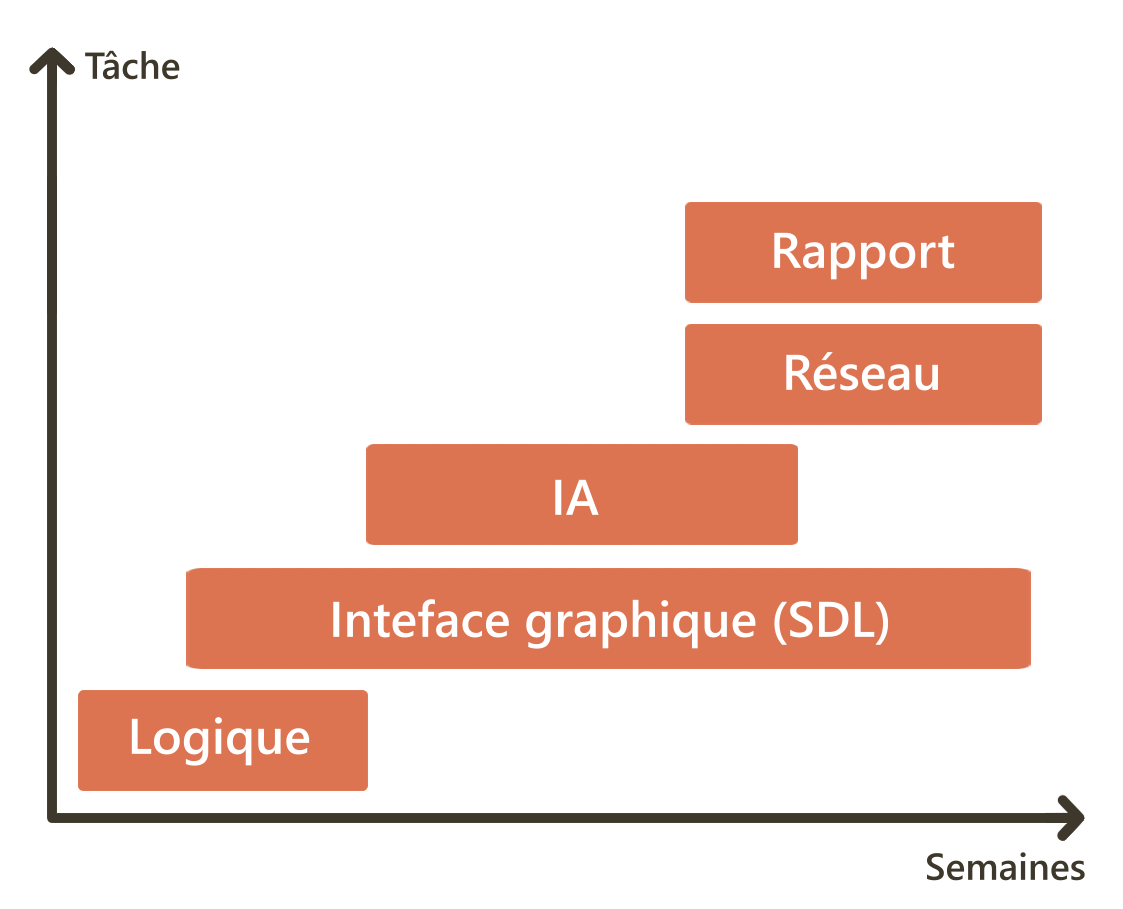
\includegraphics[height=8cm]{gantt.png}\\
            \caption{\textit{Répartition dans le temps des tâches principales}}
            \end{center}
        \end{figure}

    \subsection{Gestion des tâches et outils}
    Pour la gestion des tâches à faire, nous avons choisi d'utiliser le tableau de tickets disponible sur GitLab. Chaque ticket correspond 
    à une tâche et un responsable, et ils sont triés chronologiquement grâce à des labels; chaque label correspond à une semaine. Il
    existe aussi un label "TO DO" qui correspondait aux tâches à faire dans le futur. Au début de chaque séance, un récapitulatif de la
    semaine passée était fait; Meriem consultait chaque membre du groupe qui rendait compte de son travail depuis la séance précédente,
    puis un ticket était créé pour chaque tâche terminée. Enfin, avant de se mettre au travail, Meriem créait un nouveau label pour la
    semaine actuelle, où chacun renseignait la tâche qu'il ou elle commençait ce jour-là. \\
    
    La communication en dehors des séances de travail se faisait principalement en présentiel ou via le réseau social Discord.

\section{Développement}
    Dans cette partie, nous expliquerons en détail comment ont été implémentées toutes les fonctionnalités de notre jeu, ainsi que les fonctions et structures de données conçues. 
    \subsection{Gestion des parties}

    \subsubsection{Logique de jeu}

    La logique du jeu repose sur plusieurs mécanismes essentiels qui assurent
    le bon déroulement d’une partie d’Othello. Tout d’abord, nous avons mis
    en place une gestion simple du changement de joueur : après chaque coup,
    la couleur active alterne entre le noir et le blanc grâce à la fonction \texttt{changerJoueur}, en s’assurant que le
    joueur actuel n’est pas une valeur invalide.\\

    Ensuite, pour qu’un coup soit autorisé, il doit respecter les règles du jeu, à savoir permettre de
    capturer au moins un pion adverse. Pour cela, chaque fois qu’un joueur 
    souhaite poser un pion, la fonction \texttt{coup\_valide} vérifie dans toutes les directions
    possibles (horizontales, verticales et diagonales) s’il existe une ligne
    continue de pions adverses terminée par un pion de sa propre couleur. Si
    une telle configuration est trouvée, alors le coup est considéré comme
    valide. Ce processus de vérification est d’abord simulé sur une copie du
    plateau afin de ne pas modifier l’état du jeu tant que le coup n’est pas
    confirmé. Cela permet de préserver l'intégrité des données pendant la
    vérification. \\

    Une fois validé, les pions adverses encadrés sont retournés
    en faveur du joueur actif, ce qui reflète le cœur même de la mécanique 
    d’Othello. Le score est calculé en parcourant le plateau dans la fonction \texttt{score},
    et la boucle de jeu continue tant qu'au moins un des deux joueur peut jouer: cela est géré par la fonction \texttt{partie\_terminee}.

    \subsubsection{Sauvegarde d'une partie}
    La sauvegarde manipule des fichiers (lecture, écriture) pour enregistrer, charger ou supprimer une partie contenant le plateau, le joueur et le mode de jeu.\\
    
    Le système de sauvegarde repose sur deux structures de données \texttt{t\_case} pour le plateau et \texttt{t\_niveau} pour le mode de jeu. La fonction \texttt{chargerJeu} enregistre les pions présents sur le plateau, le joueur actuel et le mode de jeu dans un fichier texte.\\

    Nous créons un second fichier contient la liste des noms des sauvegardes disponibles, permettant de les retrouver facilement.\\

    Le chargement d'une partie consiste à lire les informations enregistrées dans le fichier correspondant. Pour reprendre la partie, les pions sont replacés aux bons emplacements sur le plateau, et les informations sur le joueur et le mode de jeu sont restaurées.\\
    
    Enfin, la possibilité de supprimer une sauvegarde est primordiale puisque le nombre de parties sauvegardées est limité à cinq. En effet, l'affichage de la liste des sauvegardes est limité par la taille de la fenêtre SDL. Ainsi la fonction \texttt{supprimer\textunderscore
    sauvegarde} efface le nom d'une partie de liste\textunderscore
    sauvegarde et supprime le fichier texte correspondant.
    

    \subsection{Mode IA}
    Le développement de l'algorithme intelligent s'est divisé en deux charges de travail : la conception de l'algorithme de décision,
    et la définition des fonctions pour l'heuristique. Ici, nous avons choisi l'algorithme Min-Max.

        \subsubsection{Algorithme MinMax}
        L'ordinateur peut jouer contre le joueur grâce à l'utilisation de l'algorithme Min-Max appliqué en profondeur. Pour cela, deux fonctionnalités principales sont mises en œuvre : une recherche récursive du meilleur coup parmi les coups possibles générés, et une autre qui détermine quel coup jouer en fonction de cette analyse. \\

        Cet algorithme repose principalement sur la structure \texttt{t\_case}, qui représente le plateau de jeu, ainsi que sur un pointeur vers une fonction heuristique permettant d'évaluer la qualité (score) de chaque coup simulé. \\
        
        La recherche récursive du meilleur coup vise à maximiser le gain de l'ordinateur tout en minimisant celui de l'adversaire. Elle simule toutes les configurations futures du plateau et attribue une valeur à chaque état à l'aide de la fonction heuristique. À chaque étape, la meilleure valeur est conservée en comparant les scores des différentes simulations.\\
        
        Comme cette recherche explore un grand nombre de possibilités, elle peut devenir très coûteuse en temps de calcul. Pour limiter cela, une profondeur maximale est définie, ce qui correspond au niveau de difficulté de l'IA : plus la profondeur est grande, plus l'I.A. est difficile à battre.\\
        
        La sélection du coup optimal est ensuite réalisée dans la fonction \texttt{minmaxChoix} en comparant les évaluations obtenues pour tous les coups valides, et en choisissant celui qui donne le meilleur résultat final. Cette approche améliore considérablement la prise de décision automatique, rendant l'IA capable de s'adapter au niveau du joueur.

        \subsubsection{Heuristique}
        Puisque notre I.A. possède plusieurs niveaux de difficulté, il fallait non seulement jouer sur la profondeur de l'arbre minmax,
        mais aussi concevoir deux fonctions d'évaluations : une "naïve", et une plus avancée. \\

        Pour la fonction d'évaluation des modes facile et moyen, nous avons décidé de concevoir une heuristique très basique qui prendrait
        des décisions de manière similaire à un débutant ayant peu d'expérience. Ainsi, la fonction \texttt{int heuristique\textunderscore
        facile(t\textunderscore
        case jeu[N][N],
        t\textunderscore
        case joueur)} n'appelle qu'une seule fonction d'évaluation: \texttt{eval\textunderscore
        score}, qui se contente de calculer la différence entre le score du
        joueur et celui de l'adversaire. \\

        Cependant, cela n'était pas suffisant pour le mode difficile; il a fallu étudier plus en détail comment gagner une partie d'Othello.
        En plus du score, trois facteurs ont été retenus: \\
            \begin{itemize}
                \item la mobilité, c'est-à-dire le nombre de coups valables pour un joueur; 
                \item les positions stratégiques sur le plateau (principalement, les quatre coins);
                \item le joueur qui posera le dernier pion.
            \end{itemize}

        Ainsi, trois fonctions supplémentaires ont été conçues pour évaluer chacun de ces points: \texttt{eval\textunderscore
        mobilite}, \texttt{eval\textunderscore
        coins} et \texttt{eval\textunderscore
        parite}.
        Toutes ces fonctions, en plus de \texttt{eval\textunderscore
        score}, sont appelées par \texttt{int heuristique\textunderscore
        avancee (t\textunderscore
        case jeu[N][N], t\textunderscore
        case joueur)}. Autrement
        dit, dans le mode difficile, l'I.A. fait en sort de maximiser son nombre de coups valables et de diminuer celui de l'adversaire, de
        capturer les quatre coins du plateau, et d'être le joueur qui posera le dernier pion (si l'I.A. joue les pions noirs, elle essaiera
        de faire sauter un tour au joueur). \\

        Afin de faciliter la création éventuelle de nouveaux modes de difficulté personnalisés, nous avons créé une fonction générale \texttt{heuristique} 
        qui prend en paramètre un plateau de jeu et un tableau de fonctions d'évaluation. \texttt{heuristique\textunderscore
        facile} et \texttt{heuristique\textunderscore
        avancee} sont simplement 
        des encapsulations de celle-ci. \\

        Des ajustements, notamment au niveau de certains coefficients, ont été apportés après lors de la phase de test de l'algorithme. \\
        
    \subsection{Interface graphique}
        Différentes fonctions ont été développées pour l’interface graphique du jeu Othello. 
        Chaque fonction a un rôle précis dans l'affichage, la gestion du plateau et du menu. \\

        \subsection{Les menus}
                Les menus permettent de naviguer entre les différentes parties du jeu : mode de jeu, paramètres, choix du niveau de l’IA, menu réseau et chargement de parties sauvegardées. Chaque menu est représenté par une valeur de l’énumération \texttt{MenuState}, ce qui facilite le passage d’un menu à un autre selon les actions du joueur. \\
        
        Pour chaque menu, une fonction d’initialisation \texttt{init\_*()} configure les éléments graphiques comme les boutons, les textes et leurs positions. Ces éléments sont stockés dans des structures comme \texttt{Button} ou \texttt{bouton\_t}, qui contiennent un rectangle \texttt{SDL\_Rect}, les couleurs normale et au survol, une texture de texte, ainsi qu’un indicateur d’état \texttt{isHovered}. Cela permet d’unifier la gestion de tous les boutons de l’interface. \\
        
        L’affichage est ensuite pris en charge par une fonction de \texttt{render\_*()} propre à chaque menu. Elle dessine les éléments à l’écran, affiche les textes et applique le bon thème (sombre ou clair) en fonction du paramètre \texttt{themeMode}. \\
        
        Les événements (clics, mouvements de la souris) sont pris en charge par des fonctions de type \texttt{handle\_*()}, qui détectent si un bouton est survolé ou cliqué. Ces fonctions modifient l’état actuel du menu \texttt{currentMenu}, activent ou désactivent des options comme le volume, ou lancent une partie selon le mode sélectionné. \\
        
        Les parties sauvegardées sont représentées par un tableau de structures \texttt{SavedGame} contenant un nom de fichier et un bouton. Cela permet de les afficher dynamiquement et de proposer des options comme le chargement ou la suppression via le bouton \texttt{btnSupprimer}. \\
 \\

        \subsection{Le plateau de jeu}
        \textbf{Structures de données et organisation du programme} \\
            Le programme utilise une matrice de jeu t\textunderscore
            case jeu[N][N] qui représente le plateau de jeu (où N est la longueur du plateau). \\

            Pour faciliter les interactions avec l'interface utilisateur, une structure "bouton" a été conçue. 
            Par ailleurs, une structure DimensionsJeu permet de stocker les dimensions de la fenêtre et des éléments de manière 
            dynamique pour s'adapter au redimensionnement. La strucure "SavedGame" contient les données des parties sauvegardées 
            comme le nom du fichier ou l'état du jeu. \\

            L'architecture du programme repose sur seize fonctions pour une meilleure modularité. \\
    
        \textbf{Gestion de l'affichage graphique} \\
            L'interface graphique, développée avec SDL2, s'appuie sur plusieurs fonctions. 
            La fonction dessinerPion() se charge du rendu visuel des pions en traçant des cercles pleins avec une complexité de O(rayon). \\

            L'affichage complet du plateau est effectué par afficherPlateau() qui initialise la grille de jeu avec les quatre pions 
            centraux initiaux. Sa complexité est quadratique car elle parcourt toute la matrice. \\

            La visualisation des coups autorisés est possible grâce à afficher\textunderscore
            coups\textunderscore
            possibles() qui affiche un cercle non plein 
            noir pour signaler les cases valides pour le joueur actuel en parcourant toutes les cases vides de la matrice et vérifiant 
            la validité du coup avec coup\textunderscore
            valide(). Sa complexité est de $O(N^4)$ dû aux vérifications des règles de l'Othello. \\

            L'affichage des scores se fait avec afficherScore(), utilisant SDL\textunderscore
            TTF pour le rendu texte. \\
    
        \textbf{Gestion des interactions utilisateur} \\
            Afin de gérer les interactions (clics souris), nous faisons appel à deux fonctions.
            gererClics() convertit les coordonnées de la souris en indices de matrice. Elle analyse les actions du joueur, 
            vérifie si le clic est dans la limite du plateau, la validité du coup, met à jour l'état du plateau et 
            gère l'alternance des tours. \\
            
            clicBouton(), quant à elle, détecte les interactions avec les éléments d'interface (comme le bouton de 
            sauvegarde par exemple) grâce à de simples comparaisons de coordonnées.\\ 

        \textbf{Gestion des parties} \\ 
            Pour gérer la logique du jeu, nous appelons la fonction principale jouerPartie() qui 
            lance une partie quel que soit le mode de jeu sélectionné (joueur contre joueur ou contre IA). Cette 
            fonction initialise les ressources SDL, gère les tours de jeu, les mises à jour de l’affichage 
            et les sauvegardes.
            Les différents modes de jeu (JoueurVsJoueur(), JoueurVsOrdi(), et leurs variantes pour les parties 
            sauvegardées) utilisent la même fonction de base (jouerPartie()), mais avec des réglages différents 
            pour lancer directement une partie selon le choix de l'utilisateur. \\
    
        \textbf{Fonctionnalités avancées} \\ 
            La gestion du temps pour chaque tour est effectuée par afficherChrono(). La fonction affiche le temps écoulé pour chaque joueur avec une icône 
            intégrée. Elle utilise la structure préexistante time\textunderscore
            t pour calculer le temps restant. \\
            L'initialisation et la libération des ressources graphiques sont prises en charge par \texttt{initialiserSDL()} 
            et \texttt{nettoyerRessources()}. Ces deux fonctions sont conçues pour s'exécuter en temps constant O(1). \\
            Enfin, l'adaptabilité aux différents formats d'écran est garantie par \texttt{mettreAJourDimensions()} qui 
            recalcule les dimensions des éléments (plateau, boutons, textes) lors du redimensionnement de la fenêtre. \\\\
            

            \subsection{Mode réseau}
    
            Le mode réseau de Othello repose sur deux principes fondamentaux : un côté serveur et un côté client. Dans les deux cas, nous utilisons les fonctions fournies par les bibliothèques réseau de sockets en langage C.
            
            Dans le processus de communication entre le serveur et le client, nous utilisons des structures de données classiques, comme celles définies dans les bibliothèques de sockets, par exemple la structure \texttt{struct sockaddr\_in}. De plus, nous réutilisons les structures propres à la gestion du jeu, notamment \texttt{t\_case jeu[N][N]}, une matrice de taille N×N représentant le plateau de jeu.
            
            
            \textbf{Serveur} \\
        
            Le serveur est considéré comme le joueur qui commence la partie. Il est donc lancé en premier. Nous utilisons la fonction \textbf{socket()} pour créer une socket TCP, que nous lions ensuite à une adresse locale à l’aide de \textbf{bind()}. Ensuite, nous plaçons la socket en écoute avec \textbf{listen()}.
            
            Le joueur serveur attend alors une connexion entrante via \textbf{accept()}. Une fois la connexion acceptée, le serveur initialise le plateau de jeu, informe le joueur qu’il jouera les pions noirs, puis la partie commence. À chaque tour, le jeu suit une logique précise : affichage du plateau, saisie du coup, mise à jour du plateau, puis envoi des données au client via \textbf{send()}. Le serveur reçoit également en retour le plateau mis à jour et d’éventuels messages de contrôle, comme "quit", grâce à \textbf{recv()}. \\
        

            \textbf{Client} \\
            
            Le client établit une connexion vers l’adresse IP du serveur à l’aide de la fonction \textbf{connect()}. Une fois la connexion établie, il reçoit l’état initial du jeu, est informé qu’il jouera les pions blancs, et attend son tour pour jouer. La logique de jeu du client est similaire à celle du serveur : il utilise \textbf{recv()} pour recevoir les mises à jour et \textbf{send()} pour envoyer les coups joués. \\
        

            \textbf{Synchronisation} \\

            Le bon déroulement de la partie repose sur un ensemble de fonctions essentielles : \texttt{init\_jeu()}, \texttt{afficher\_jeu()}, \texttt{placer\_pion()} et \texttt{changerJoueur()}. Chaque action du joueur est validée avant d’être exécutée. Par exemple, la fonction \texttt{peut\_jouer()} vérifie si un joueur peut jouer, et \texttt{partie\_terminee()} détermine si la partie est terminée.
        
            L’échange de données entre les deux joueurs est strictement alterné, ce qui garantit une bonne synchronisation. À chaque tour, deux éléments sont transmis :
        
            - Le plateau de jeu (\textbf{jeu})
        
            - Un joueur actif  (\textbf{joueur\_actif}), pour savoir le tour de quel joueur de jouer. \\
            

            \textbf{Connexion} \\
        
            Pour assurer une transmission fiable des données, nous avons choisi le protocole TCP. Afin de jouer entre deux machines (client-serveur), l’utilisateur doit entrer l’adresse IP du serveur. Ce choix permet une communication stable, avec un contrôle d’erreur intégré, garantissant que les données soient correctement envoyées et reçues.
            
            \begin{center}
                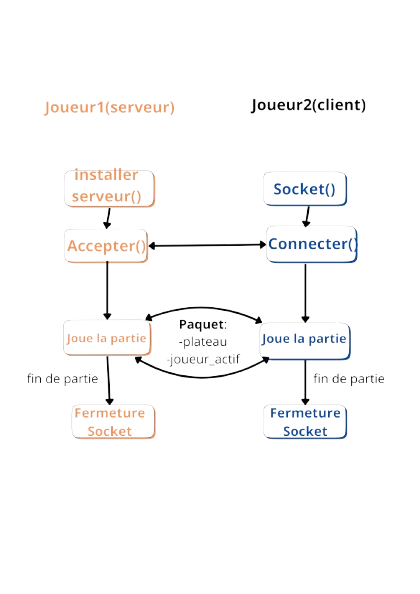
\includegraphics[scale=0.7]{schema_reseau.png}
            \end{center}

\section{Conclusion}


Les objectifs que nous nous étions fixés ont été atteints. A l'origine, nous voulions concevoir un jeu Othello jouable en mode hotseat ou contre une intelligence artificielle. Finalement, nous avons avancé plus vite que prévu, ce qui nous a permis d'aller plus loin et d'implémenter un mode multijoueur en ligne. De ce point de vue, les objectifs originaux ont été dépassés. \\

Cependant, cela ne s'est pas fait sans difficultés. De nombreux imprévus ont mis à l'épreuve notre organisation, autant des absences que des pannes de matériel. Nous avons été poussés à revoir nos priorités, sacrifiant certaines fonctionnalités au profit d'autres plus importantes. Par exemple, l'amélioration du système de sauvegarde a été privilégiée à l'élagage alpha-beta de min-max. Ceci eut un impact considérable sur le déroulement du projet. \\

Notre plan prévisionnel (disponible en annexe) se retrouve assez éloigné de la réalité; nous avons surestimé le temps que prendraient certaines tâches (comme l'interface graphique), et inversement. De plus, nous n'avons pas pris en compte les imprévus possibles, ainsi que les difficultés de coordination qu'apporte le travail en groupe. \\

Grâce à une bonne communication et aux outils collaboratifs efficaces à notre disposition, le projet a pu être mené à terme. Cette expérience nous a permis d’améliorer nos compétences techniques, ainsi que de tirer des leçons importantes en gestion de projet et en travail d’équipe.

\newpage 
\section{Annexe}
    \textbf{Jeu de test pour la fonction score (scr/jeu/fonc\textunderscore
    jeu.c):}

    N x N est la dimension du plateau (usuellement N = 8) \\

    Plateau de jeu plein
    \begin{itemize} 
        \item de pions blancs (résultat attendu: score(blanc) = N*N, score(noir) = 0, score(vide) = 0),
        \item de pions noirs (résultat attendu: score(noir) = N*N, score(blanc) = 0, score(vide) = 0);
    \end{itemize} 

    Plateau de jeu vide (résultat attendu: score(noir) = score(blanc) = 0, score(vide) = N*N);

    Plateau de jeu avec seulement bords pleins:
    \begin{itemize}
        \item bords blancs (résultat attendu: score(blanc) = N*N - (N-2) * (N-2), score(noir) = 0, score(vide) = (N-2) * (N-2)),
        \item bords noirs (résultat attendu: score(noir) = N*N - (N-2) * (N-2), score(blanc) = 0, score(vide) = (N-2) * (N-2));
    \end{itemize} \\
    
    Plateau de jeu avec seulement coins pleins:
    \begin{itemize}
        \item coins blancs (résultat attendu: score(blanc) = 4, score(noir) = 0, score(vide) = N*N - 4),
        \item coins noirs (résultat attendu: score(noir) = 4, score(blanc) = 0, score(vide) = N*N - 4);
    \end{itemize}

\newpage


    \textbf{Exemple de débuggage}
    
    Nous avons rencontré un bug lors de la conception de l'interface graphique pour jouer contre l'IA. Choisir le mode difficile
    renvoyait une erreur de segmentation. Voici comment nous avons repéré le bug avec le débuggeur gdb:

    \begin{center}
        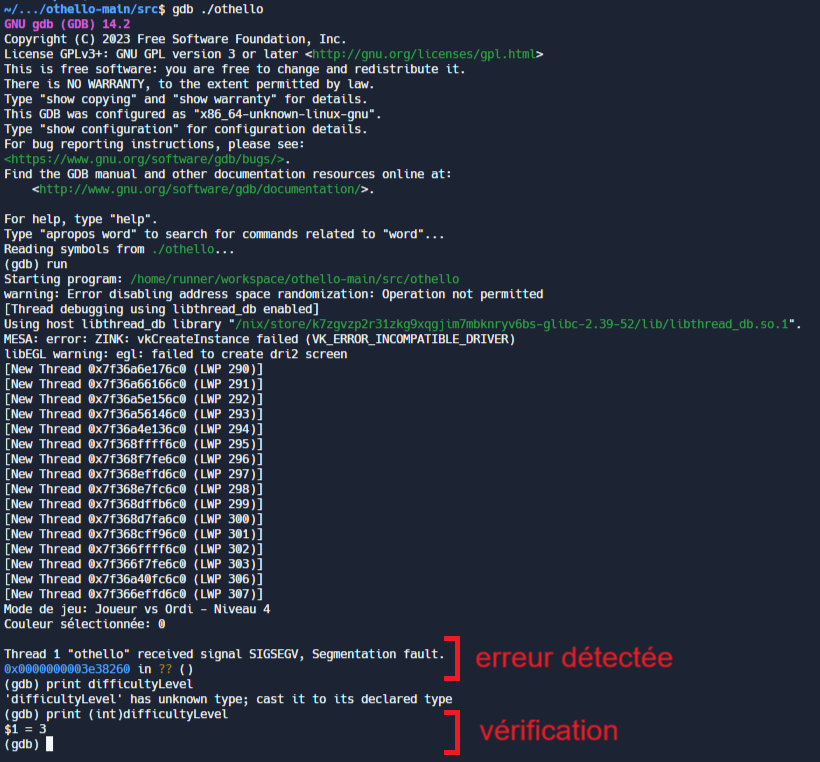
\includegraphics[scale=0.7]{gdb.png}
    \end{center}

    Le problème se trouvait dans la valeur attribuée à difficultyLevel. Les valeurs étaient passées "en dur" au lieu d'utiliser
    l'énumération t\_niveau.

    \begin{center}
        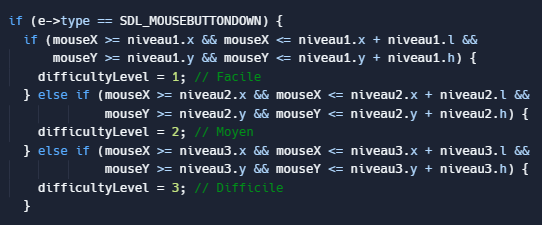
\includegraphics[scale=0.7]{erreur.png}
    \end{center}

    Ceci posait problème car t\_niveau était définit ainsi à cette phase du projet:

    \begin{center}
        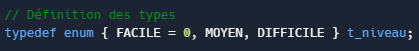
\includegraphics[scale=0.7]{tniveau.png}
    \end{center}

    Nous avons donc corrigé le bug en attribuant les bonnes valeurs à difficultyLevel.
    
    \begin{center}
        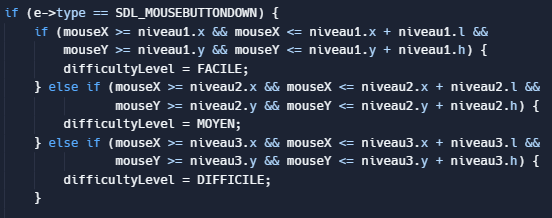
\includegraphics[scale=0.7]{erreur_corrigee.png}
    \end{center}

\newpage

    \textbf{Captures d'écran}
        \begin{center}
            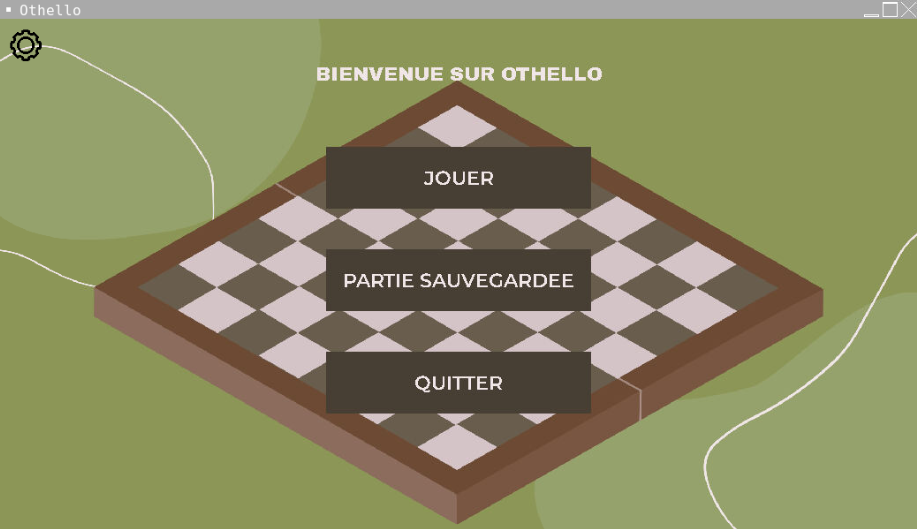
\includegraphics[scale=0.7]{menu_principal.png}
            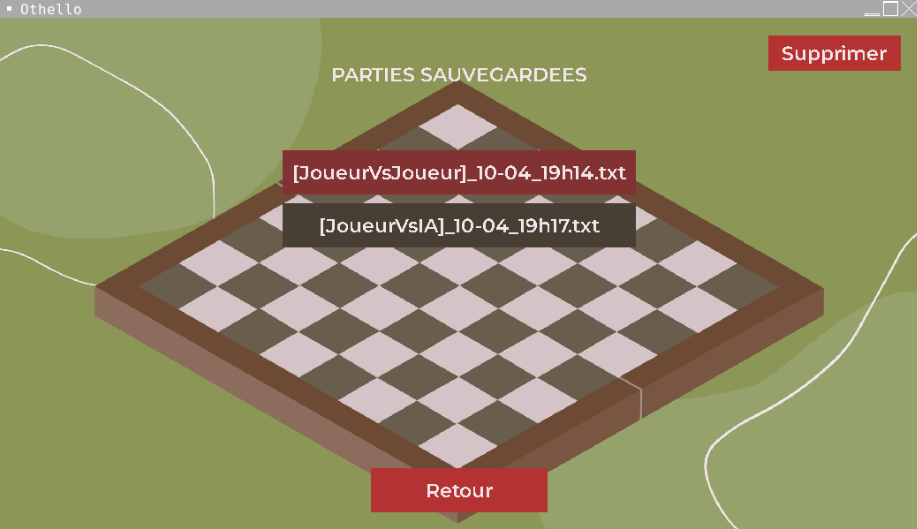
\includegraphics[scale=0.7]{menu_sauv.png}
            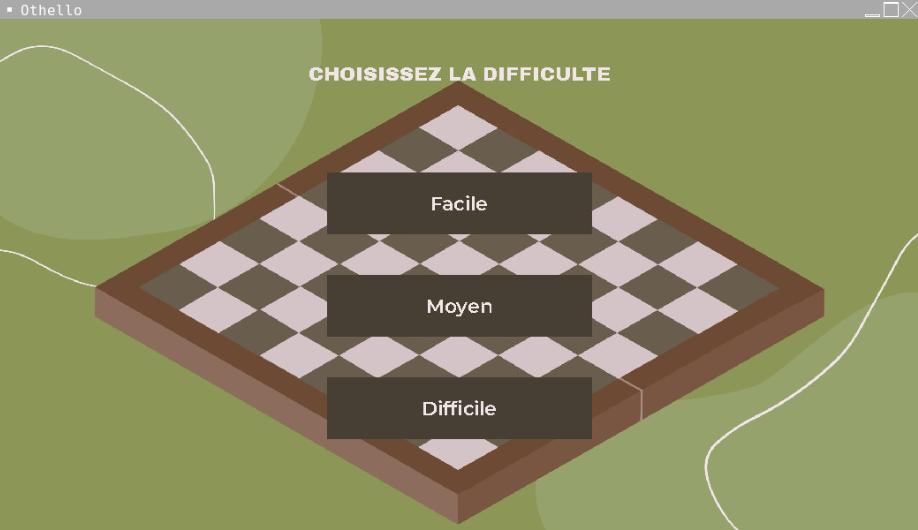
\includegraphics[scale=0.7]{sous_menu.png}
            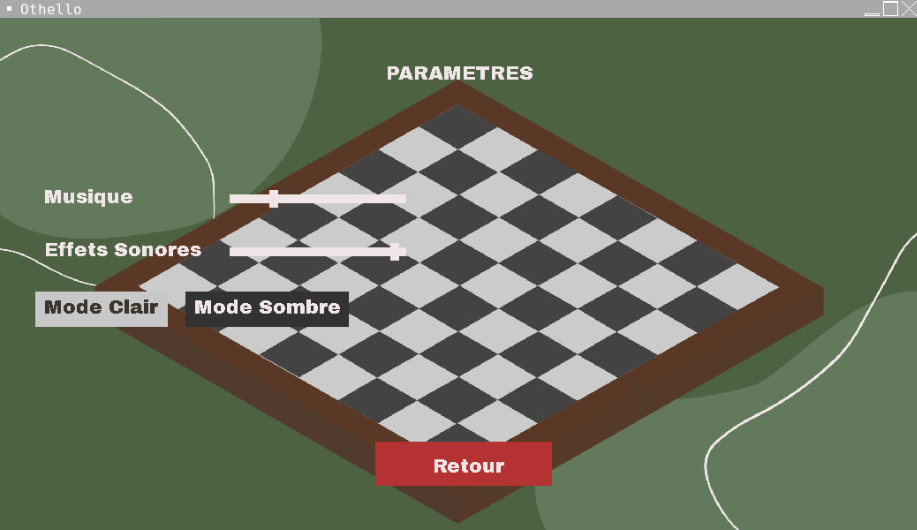
\includegraphics[scale=0.7]{parametres.png}
            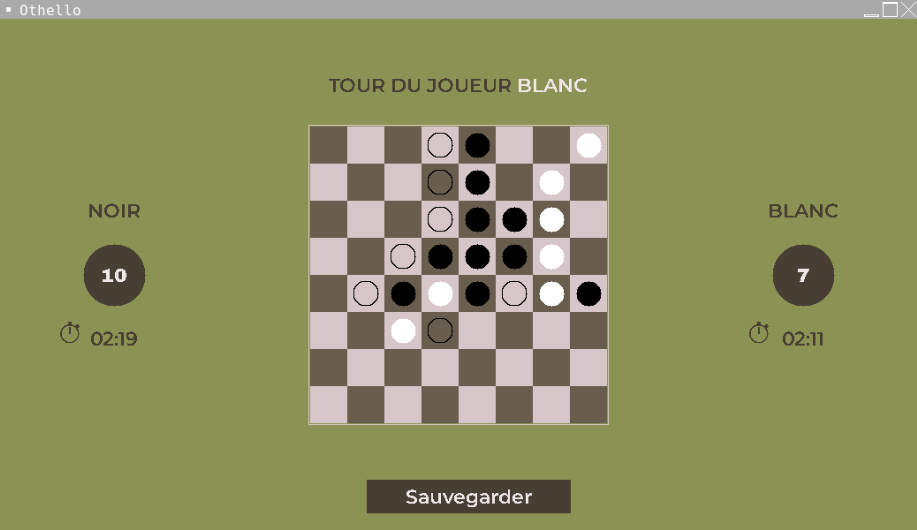
\includegraphics[scale=0.7]{partie.png}
        \end{center}


\end{document}
